\documentclass[nooutcomes]{ximera}
\input{../preamble}


\author{Bobby Ramsey}
\license{Creative Commons Attribution 4.0 International License}
\acknowledgement{https://github.com/mooculus/calculusWithReview}

\title{Solving Trigonometric Equations}
% Learning Objectives for this section
%\begin{itemize}
%	\item Degrees and Radians
%	\item Reference Angles
%	\item The Definition of trigonometric functions in terms of the Unit Circle 
%	\item Evaluating trigonometric functions at standard angles
%\end{itemize}


\begin{document}

\begin{abstract}
	
\end{abstract}
\maketitle


%\typeout{************************************************}
%\typeout{Review Questions}
%\typeout{************************************************}

%\section{Review Materials}
%    \begin{itemize}[label=\textbullet]
%	\item \link[Combining Like Terms]{https://spot.pcc.edu/math/orcca/ed2/html/section-combining-like-terms.html}
%	\item \link[Algebraic Properties and Simplifying Expressions]{https://spot.pcc.edu/math/orcca/ed2/html/section-algebraic-properties-and-simplifying-expressions.html}
%   \end{itemize}
%\begin{motivatingQuestions}\begin{itemize}
	%Often start a section. 
%	\item How can we define trigonometric functions for angles that do not come from triangles?
%\end{itemize}\end{motivatingQuestions}

\section{Introduction}

Frequently we are in the situation of having to determine precisely which angles satisfy a particular equation. Something like $\sin(\theta) = \frac{\sqrt{2}}{2}$. We know that $\sin\left( \frac{\pi}{4} \right) = \frac{\sqrt{2}}{2}$, meaning that $\theta = \frac{\pi}{4}$ is a solution of this equation, but is that the only solution or \emph{are there more}?

Let's look at the graph of the sine function.
\begin{image}
\begin{tikzpicture}
	\begin{axis}[
            xmin=-6.75,xmax=6.75,ymin=-1.5,ymax=1.5,
            axis lines=center,
            xtick={-6.28, -4.71, -3.14, -1.57, 0, 1.57, 3.142, 4.71, 6.28},
            xticklabels={$-2\pi$,$-3\pi/2$,$-\pi$, $-\pi/2$, $0$, $\pi/2$, $\pi$, $3\pi/2$, $2\pi$},
            ytick={-1,1},
            minor ytick=,minor xtick=,
            width=6in,
            height=3in,
            unit vector ratio*=1 1 1,
            every axis y label/.style={at=(current axis.above origin),anchor=south},
            every axis x label/.style={at=(current axis.right of origin),anchor=west},
          ]        
          \addplot [very thick, penColor, samples=300,smooth, domain=(-6.75:6.75)] {sin(deg(x))} node[pos=0.65, penColor, right, thick] {\large{$y=\sin(\theta)$}};
	\addplot[ thick, penColor2, domain=(-6.75:6.75)]{0.707} node[pos=0.33, above,penColor2, thick]{$y=\frac{\sqrt{2}}{2}$};
        \end{axis}
\end{tikzpicture}
\end{image}
Notice that the graph of $\sin(\theta)$ and the graph of the constant function $y=\frac{\sqrt{2}}{2}$ intersect many times, not just once. In fact, since sine is a
periodic function, these graphs intersect infinitely many times. Each of these intersections represents a single solution of the equation $\sin(\theta) = \frac{\sqrt{2}}{2}$. We need a process to identify and write down each of these solutions. Let's start by looking at the unit circle. Remember that sine values
correspond to the $y$-coordinate of points on the unit circle. This equation is asking us to find all the points on the unit circle with a $y$-coordinate of
$\frac{\sqrt{2}}{2}$.

\begin{image}
\begin{tikzpicture}
	\begin{axis}[
            xmin=-1.1,xmax=1.1,ymin=-1.1,ymax=1.1,
            axis lines=center,
            width=4in,
            xtick={-1,1},
            ytick={-1,1},
            clip=false,
            unit vector ratio*=1 1 1,
            xlabel=$x$, ylabel=$y$,
            every axis y label/.style={at=(current axis.above origin),anchor=south},
            every axis x label/.style={at=(current axis.right of origin),anchor=west},
          ]        
          \addplot [dashed, smooth, domain=(0:360)] ({cos(x)},{sin(x)}); %% unit circle


          \addplot+[thick,penColor,->] plot coordinates {(0,0) (.707,.707)}; %% 40 degrees
          \addplot+[thick,penColor2,->] plot coordinates {(0,0) (-.707,.707)}; %% 40 degrees
%          \addplot+[thick,penColor3,->] plot coordinates {(0,0) (-.766,-.643)}; %% 40 degrees
%          \addplot+[thick,penColor4,->] plot coordinates {(0,0) (.766,-.643)}; %% 40 degrees
          
          \addplot+[thick,penColor,->] plot coordinates {(0,0) (1,0)}; %% 40 degrees
          
          \addplot [penColor,smooth, domain=(0:45)] ({.1*cos(x)},{.1*sin(x)});
          \addplot [penColor2,smooth, domain=(0:135)] ({.15*cos(x)},{.15*sin(x)});
%          \addplot [penColor3,smooth, domain=(0:220)] ({.2*cos(x)},{.2*sin(x)});
%          \addplot [penColor3,smooth, domain=(0:320)] ({.25*cos(x)},{.25*sin(x)});

	\addplot[thick, penColor3, domain=(-1.1:1.1)]{0.707} node[pos=0.4, above]{$y=\frac{\sqrt{2}}{2}$};          
         \end{axis}
\end{tikzpicture}
\end{image}
You see that there are two locations on the unit circle with $y$-coordinate equal to $\frac{\sqrt{2}}{2}$, one in the first quadrant and another in the second.
As we mentioned earlier, the first quadrant angle is $\theta = \frac{\pi}{4}$. The angle in the second quadrant has reference angle $\frac{\pi}{4}$, which 
means the angle is $\frac{3\pi}{4}$. Those are the only two points on the circle with that $y$-coordinate, but remember that there are many other angles
which are coterminal with those. For instance:
\begin{image}
\begin{tikzpicture}
	\begin{axis}[
            xmin=-1.1,xmax=1.1,ymin=-1.1,ymax=1.1,
            axis lines=center,
            width=4in,
            xtick={-1,1},
            ytick={-1,1},
            clip=false,
            unit vector ratio*=1 1 1,
            xlabel=$x$, ylabel=$y$,
            every axis y label/.style={at=(current axis.above origin),anchor=south},
            every axis x label/.style={at=(current axis.right of origin),anchor=west},
          ]        
          \addplot [dashed, smooth, domain=(0:360)] ({cos(x)},{sin(x)}); %% unit circle


          \addplot+[thick,penColor,->] plot coordinates {(0,0) (.707,.707)}; %% 40 degrees
%          \addplot+[thick,penColor2,->] plot coordinates {(0,0) (-.707,.707)}; %% 40 degrees
%          \addplot+[thick,penColor3,->] plot coordinates {(0,0) (-.766,-.643)}; %% 40 degrees
%          \addplot+[thick,penColor4,->] plot coordinates {(0,0) (.766,-.643)}; %% 40 degrees
          
          \addplot+[thick,penColor,->] plot coordinates {(0,0) (1,0)}; %% 40 degrees
          
          \addplot [penColor,smooth, domain=(0:405)] ({(.1+0.1*x/405)*cos(x)},{(.1+0.1*x/405)*sin(x)});
 %        \addplot [penColor2,smooth, domain=(0:135)] ({.15*cos(x)},{.15*sin(x)});
%          \addplot [penColor3,smooth, domain=(0:220)] ({.2*cos(x)},{.2*sin(x)});
%          \addplot [penColor3,smooth, domain=(0:320)] ({.25*cos(x)},{.25*sin(x)});

	\addplot[thick, penColor3, domain=(-1.1:1.1)]{0.707} node[pos=0.4, above]{$y=\frac{\sqrt{2}}{2}$};          
         \end{axis}
\end{tikzpicture}
\end{image}

The only solutions are the angles $\frac{\pi}{4}$, $\frac{3\pi}{4}$, and \emph{all the angles coterminal with them}. Since the sine function has period
$2\pi$, that means any other solution has to be an integer multiple of $2\pi$ away from one of these first two solutions. Putting that together, our solutions
are:
$$ \theta = \frac{\pi}{4} + 2\pi k , \,\, \frac{3\pi}{4}+2\pi k , \,\, k \textrm{ any integer}. $$

The steps we've followed are summarized in the following.
\begin{callout}
	To solve a triginometric equation:
	\begin{enumerate}
		\item Find the reference angle of the solutions. Typically the standard values will help identify this.
		\item Find all solutions on a single period of the function. Use the graph, the unit circle, and the reference angle to identify these.
		\item Find all solutions. Use the period of the function to find all requested solutions.
	\end{enumerate}
\end{callout}


\begin{example}
	Solve the equation: \[ \sin(\theta) = -\frac{1}{2}. \]
	\begin{explanation}
		We'll start by finding the reference angle, $\theta_R$, the acute angle between the terminal side of $\theta$ and the $x$-axis.  
		The reference angle satisfies $\sin(\theta_R) = \frac{1}{2}$ and the negative sign will be used to indicate the quadrant of the angle.
		\begin{image}[2in]
		   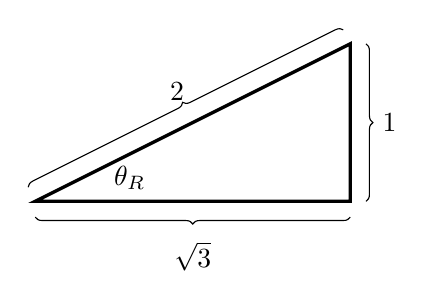
\begin{tikzpicture}
    			\coordinate (C) at (0,2);
    			\coordinate (D) at (4,2);
   			 \coordinate (E) at (4,4);
   			 %\tkzMarkRightAngle(C,D,E)
    			%\tkzMarkAngle(D,C,E)
    			\draw[decoration={brace,mirror,raise=.2cm},decorate,thin] (0,2)--(4,2);
   			 \draw[decoration={brace,mirror,raise=.2cm},decorate,thin] (4,2)--(4,4);
  			  \draw[decoration={brace,raise=.2cm},decorate,thin] (0,2)--(4,4);
  			  \draw[very thick] (D)--(E)--(C)--cycle;
    			\node at (2,2-.7) {$\sqrt{3}$};
    			\node[] at (4+.5,3) {$1$};
    			\node at (2-.2,3+.4) {$2$};
    			\node at (1.2,2.3) {$\theta_R$};
  		  \end{tikzpicture}
		\end{image}
		From the picture we see $\theta_R = \frac{\pi}{6}$.  Let's look at the unit circle.
		
		\begin{image}
\begin{tikzpicture}
	\begin{axis}[
            xmin=-1.1,xmax=1.1,ymin=-1.1,ymax=1.1,
            axis lines=center,
            width=4in,
            xtick={-1,1},
            ytick={-1,1},
            clip=false,
            unit vector ratio*=1 1 1,
            xlabel=$x$, ylabel=$y$,
            every axis y label/.style={at=(current axis.above origin),anchor=south},
            every axis x label/.style={at=(current axis.right of origin),anchor=west},
          ]        
          \addplot [dashed, smooth, domain=(0:360)] ({cos(x)},{sin(x)}); %% unit circle


          \addplot+[thick,penColor2,->] plot coordinates {(0,0) (.5,-0.866)}; %% 40 degrees
          \addplot+[thick,penColor,->] plot coordinates {(0,0) (-.5,-0.866)}; %% 40 degrees
          \addplot+[thick,penColor,->] plot coordinates {(0,0) (1,0)}; %% 40 degrees
          
          \addplot [penColor,smooth, domain=(0:240)] ({0.1*cos(x)},{0.1*sin(x)});
          \addplot [penColor2,smooth, domain=(0:300)] ({0.15*cos(x)},{0.15*sin(x)});
  	  \addplot[thick, penColor3, domain=(-1.1:1.1)]{-0.866} node[pos=0.4, below]{$y=\frac{\sqrt{3}}{2}$};          
         \end{axis}
\end{tikzpicture}
\end{image}

In one period $[0, 2\pi)$, there are two angles that have reference angle $\frac{\pi}{6}$ and have negative
		sine value.  One is in quadrant 3, and one in quadrant 4.  That means the solutions in the interval $[0, 2\pi)$ are $\frac{7\pi}{6}$ and $\frac{11\pi}{6}$.
		
		To find all solutions, we have to add all multiples of $2\pi$ to these.  The solutions are then $$ \theta = \frac{5\pi}{6} + 2\pi k , \,\, \frac{11\pi}{6}+2\pi k , \,\, k \textrm{ any integer}. $$
	\end{explanation}
\end{example}

\begin{example}
	Solve the equation: \[ \tan(\theta) = -\sqrt{3}. \]

	\begin{explanation}
		We'll start by finding the reference angle, $\theta_R$, the acute angle between the terminal side of $\theta$ and the $x$-axis.  
		The reference angle satisfies $\tan(\theta_R) = \sqrt{3}$ and the negative sign will be used to indicate the quadrant of the angle.
		Since tangent is opposite over adjacent, we have the following triangle.
		\begin{image}[2in]
		   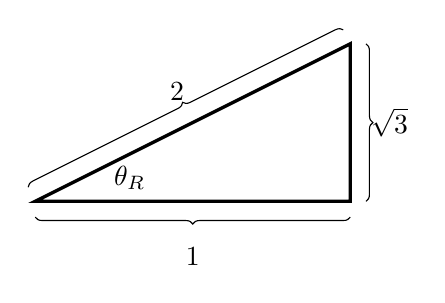
\begin{tikzpicture}
    			\coordinate (C) at (0,2);
    			\coordinate (D) at (4,2);
   			 \coordinate (E) at (4,4);
   			 %\tkzMarkRightAngle(C,D,E)
    			%\tkzMarkAngle(D,C,E)
    			\draw[decoration={brace,mirror,raise=.2cm},decorate,thin] (0,2)--(4,2);
   			 \draw[decoration={brace,mirror,raise=.2cm},decorate,thin] (4,2)--(4,4);
  			  \draw[decoration={brace,raise=.2cm},decorate,thin] (0,2)--(4,4);
  			  \draw[very thick] (D)--(E)--(C)--cycle;
    			\node at (2,2-.7) {$1$};
    			\node at (4+.5,3) {$\sqrt{3}$};
    			\node at (2-.2,3+.4) {$2$};
    			\node at (1.2,2.3) {$\theta_R$};
  		  \end{tikzpicture}
		\end{image}
		From the picture we see $\theta_R = \frac{\pi}{3}$.		
	
		The tangent function goes through one period on the interval $\left( -\frac{\pi}{2}, \frac{\pi}{2}\right)$. In the interval $\left( -\frac{\pi}{2}, 0\right)$ 
		(which is Quadrant IV), tangent is negative while in $\left( 0, \frac{\pi}{2}\right)$ (which is Quadrant I), tangent is positive.
		For $\tan(\theta)$ to be negative in this interval, we need $\theta$ to be in $\left( -\frac{\pi}{2}, 0\right)$. The only angle in
		that interval with reference angle $\frac{\pi}{3}$ is $\theta = -\frac{\pi}{3}$. This is the only solution on this period.
		\begin{callout}
			Remember that the tangent function has period $\pi$, unlike sine and cosine which have period $2\pi$. On the period
			$\left( -\frac{\pi}{2}, \frac{\pi}{2}\right)$, tangent is one-to-one, so there is exactly one angle which gives the desired
			output value. Sine and cosine are not one-to-one across a full period.
		\end{callout}
		
		To find all solutions, we have to add all multiples of $\pi$ to this.  
		The solutions are then $$ \theta = -\frac{\pi}{3}+ \pi k , \,\, k \textrm{ any integer}. $$
				
	\end{explanation}
\end{example}

Let's try one a bit more complicated.
\begin{example}
	Solve the equation: \[ \cos(\theta) \left( \cos(\theta) + 1\right) = \sin^2(\theta). \]
	\begin{explanation}
		We'll start by simplifying a bit. Note that we use a rearranged form of the Pythagorean identity, $\sin^2(\theta)  = 1 - \cos^2(\theta)$. 
		\begin{align*}
			\cos(\theta) \left( \cos(\theta) + 1\right) &= \sin^2(\theta) \\
			\cos^2(\theta) + \cos(\theta) &= \sin^2(\theta) \\
			\cos^2(\theta) - \sin^2(\theta) + \cos(\theta) &= 0\\
			\cos^2(\theta) - \left(1-\cos^2\theta\right) + \cos(\theta) &= 0\\
			2\cos^2(\theta) + \cos(\theta) - 1 &= 0.
		\end{align*}
		Notice that this equation is quadratic in $\cos(\theta)$.  We can factor it like we try to do to solve any other quadratic equation:
		\[ \left( \cos(\theta) + 1 \right) \left( 2 \cos(\theta) - 1\right) = 0.\]
		Now, we can set each factor equal to zero and solve the two resulting equations:
		$$\cos(\theta) + 1 = 0 \text{ and } 2\cos(\theta) - 1 = 0$$
		yield the equations $\cos(\theta) = -1$ and $\cos(\theta) = \frac{1}{2}$. 
		On the interval $[0, 2\pi)$, $\cos(\theta) = -1$ has only one solution, $\theta = {\pi}$.  
		For $\cos(\theta) = \frac{1}{2}$, we see that the reference angle $\theta_R = {\frac{\pi}{3}}$.  Since cosine is positive in Quadrants I and IV,
		we find solutions $\theta = \frac{\pi}{3}$ and $\frac{5\pi}{3}$.
		
		All solutions are:
		\[ \theta = \pi + 2 \pi k, \,\, \frac{\pi}{3}+ 2 \pi k ,\,\, \frac{5\pi}{3} + 2\pi k, \,\, k \textrm{ any integer.} \]
	\end{explanation}
\end{example}


\end{document}
